\documentclass[a4paper,11pt,oneside]{amsbook}

\usepackage[rgb]{xcolor}
\usepackage{comments}
\usepackage{booktabs}
\usepackage[T1]{fontenc}
\usepackage{lmodern}
\usepackage{microtype}
\usepackage{amssymb}
\usepackage{amsrefs}
\usepackage{enumitem}
\usepackage{graphicx}
\usepackage{subcaption}
\usepackage{pdfpages}
\usepackage{hyperref}
\usepackage[capitalise,noabbrev]{cleveref}
\usepackage{etoolbox}
\usepackage{pgfkeys}
\usepackage{minted}
\usepackage{tikz}
\usepackage{newfloat}
\usepackage[noend,noline,linesnumbered]{algorithm2e}
\usepackage{xparse}
\usepackage{chngcntr}
\usepackage{lipsum}

%\usepackage{showframe}

% less aggressive hyperlinks
\hypersetup{%
  pdfborderstyle={/S/U/W 1}, % underline links instead of boxes
  linkbordercolor=red,       % color of internal links
  citebordercolor=green,     % color of links to bibliography
  filebordercolor=magenta,   % color of file links
  urlbordercolor=cyan        % color of external links
}
% since I refer to listings across sections
\counterwithin{listing}{section}
\counterwithin{figure}{section}

% tikz setup
\usetikzlibrary{arrows,fit,positioning,matrix,calc,scopes,chains,tikzmark}

% example environment
\newtheorem{example}{Example}[section]

% temporal operators
\makeatletter
\input pdf-trans
\newbox\qbox
\def\usecolor#1{\csname\string\color@#1\endcsname\space}
\newcommand\outline[1]{\leavevmode%
  \def\maltext{#1}%
  \setbox\qbox=\hbox{\maltext}%
  \boxgs{Q q 2 Tr .3\space w \fillcol\space \bordercol\space}{}%
  \copy\qbox%
}
\makeatother

\newcommand\colsplit[2]{\colorlet{tmpcolor}{#2}\edef\tmp{\usecolor{tmpcolor}}%
  \def\tmpB{}\expandafter\colsplithelp\tmp\relax%
  \ifnum0=#1\relax\edef\fillcol{\tmpB}\else\edef\bordercol{\tmpC}\fi}
\def\colsplithelp#1#2 #3\relax{%
  \edef\tmpB{\tmpB#1#2 }%
  \ifnum `#1>`9\relax\def\tmpC{#3}\else\colsplithelp#3\relax\fi
}
\colsplit{1}{black}
\colsplit{0}{white}

\DeclareFontFamily{U}{mathb}{\hyphenchar\font45}
\DeclareFontShape{U}{mathb}{m}{n}{
      <5> <6> <7> <8> <9> <10> gen * mathb
      <10.95> mathb10 <12> <14.4> <17.28> <20.74> <24.88> mathb12
      }{}
\DeclareSymbolFont{mathb}{U}{mathb}{m}{n}

\DeclareFontFamily{U}{matha}{\hyphenchar\font45}
\DeclareFontShape{U}{matha}{m}{n}{
      <5> <6> <7> <8> <9> <10> gen * matha
      <10.95> matha10 <12> <14.4> <17.28> <20.74> <24.88> matha12
      }{}
\DeclareSymbolFont{matha}{U}{matha}{m}{n}

\makeatletter
\newcommand{\superimpose}[2]{%
  {\ooalign{$#1\@firstoftwo#2$\cr\hfil$#1\@secondoftwo#2$\hfil\cr}}}
\newcommand{\raisemath}[1]{\mathpalette{\raisem@th{#1}}}
\makeatother

\DeclareMathSymbol{\nextP}{\mathbin}{matha}{"0D}
\DeclareMathSymbol{\nextF}{\mathbin}{matha}{"05}
\newcommand{\nextWP}{\mathbin{\hat{\nextP}}}
\newcommand{\nextWF}{\mathbin{\hat{\nextF}}}
\DeclareMathSymbol{\alwaysPP}{\mathbin}{mathb}{"0D}
\newcommand{\alwaysP}{\mathbin{\mathpalette\superimpose{{\alwaysPP}{\alwaysF}}}}
\DeclareMathSymbol{\alwaysF}{\mathbin}{mathb}{"05}
\DeclareMathSymbol{\eventuallyPP}{\mathbin}{mathb}{"0C}
\newcommand{\eventuallyP}{\mathbin{\mathpalette\superimpose{{\eventuallyPP}{\eventuallyF}}}}
\DeclareMathSymbol{\eventuallyF}{\mathbin}{matha}{"0C}
\newcommand{\triggerP}{\mathbin{\mathpalette\superimpose{{\alwaysP}{\textcolor{white}{\cdot}}}}}
\newcommand{\triggerF}{\mathbin{\mathpalette\superimpose{{\alwaysF}{\cdot}}}}
\newcommand{\sinceF}{\mathbin{\mathpalette\superimpose{{\eventuallyF}{\cdot}}}}
\newcommand{\sinceP}{\mathbin{\mathpalette\superimpose{{\eventuallyP}{\textcolor{white}{\cdot}}}}}
\newcommand{\initialP}{\mbox{\bfseries\sffamily I}}
\newcommand{\initialF}{\outline{\bfseries\sffamily F}}
\newcommand\initiallyNP{{\hat{\eventuallyP}}}
\newcommand\initiallyP[1]{{\hat{\eventuallyP} #1}}
\newcommand\initiallyNF{{\hat{\eventuallyF}}}
\newcommand\initiallyF[1]{{\hat{\eventuallyF} #1}}

% breaks in align environment
\newenvironment{alignbr*}{\allowdisplaybreaks\csname align*\endcsname}{\csname endalign*\endcsname}

% operations on states in multi-shot section
\newenvironment{StateOp}{%
\newcommand\opitem[1]{%
\renewcommand\makelabel[1]{####1}
\item[##1]\leavevmode\\}
\description[font=\normalfont,leftmargin=2em]}{%
\enddescription}

% restyle algorithm environment
% (makes it look similar to the listings environment)
\DontPrintSemicolon
\SetStartEndCondition{ }{}{}%
\SetKwComment{tcp}{\#~}{}
\SetKwProg{Fn}{function}{:}{end}
\SetKw{KwTo}{in}
\SetKwFor{For}{for}{\string:}{}%
\SetKwIF{If}{ElseIf}{Else}{if}{:}{else if}{else:}{}%
\SetKwFor{While}{while}{:}{fintq}%
\SetKwFor{ForEach}{for each}{:}{fintq}%
\AlgoDontDisplayBlockMarkers\SetAlgoNoEnd\SetAlgoNoLine%
\setlength{\algomargin}{\leftskip}
\addtolength{\algomargin}{\parskip}
\SetNlSkip{1em}
\SetNlSty{}{}{}
\let\savedalgorithm\algorithm
\let\savedendalgorithm\endalgorithm
\newenvironment{algorithm2e}{%
\renewenvironment{algocf}[1][h]{}{}%
\savedalgorithm}{%
\savedendalgorithm}
\DeclareFloatingEnvironment[name=Algorithm]{algorithmf}
\renewenvironment{algorithm}{%
\algorithmf\raggedright}{%
\endalgorithmf}
\Crefname{algorithmf}{Algorithm}{Algorithms}
\Crefname{algocfline}{Line}{Lines}

% support for nested listings
\DeclareCaptionSubType{listing}
\captionsetup[sublisting]{labelformat=parens}
\Crefname{sublisting}{Listing}{Listings}

\renewcommand{\thesection}{\thechapter.\arabic{section}}
\makeatletter
\def\@seccntformat#1{%
  \protect\textup{\protect\@secnumfont
    \csname the#1\endcsname\enspace
  }%
}
\renewcommand{\tocsection}[3]{%
  \indentlabel{\@ifnotempty{#2}{\ignorespaces#1 #2\quad}}#3}
\makeatother

\newsavebox{\mintedbox}
\NewDocumentEnvironment{mintedsubcaptionbox}{O{#2}mO{}m}{%
  \VerbatimEnvironment%
  \RecustomVerbatimEnvironment{Verbatim}{BVerbatim}{}%
  \begin{lrbox}{\mintedbox}%
  \begin{minted}[escapeinside=||,#3]{#4}}{%
  \end{minted}%
  \end{lrbox}%
  \subcaptionbox[#1]{#2}[.5\linewidth]{\usebox{\mintedbox}}}

\newcommand\inputmintedsubcaptionbox[3]{%
  \RecustomVerbatimEnvironment{Verbatim}{BVerbatim}{}%
  \begin{lrbox}{\mintedbox}%
  \inputminted[escapeinside=\%\#]{#2}{#3}%
  \end{lrbox}%
  \subcaptionbox{#1}[.49\linewidth]{\usebox{\mintedbox}}}

% line refs with the minted package
\newcommand\llabel[1]{\label[line]{#1}\hypertarget{#1}{}}
\newcommand\Lref[1]{Line~\hyperlink{#1}{\ref*{#1}}}
\newcommand\lref[1]{\Lref{#1}}
\newcommand\Lrefrange[2]{Lines~\hyperlink{#1}{\ref*{#1}} to~\hyperlink{#2}{\ref*{#2}}}
\newcommand\lrefrange[2]{\Lrefrange{#1}{#2}}

\makeatletter
\newcounter{lrefs@count}%
\newcounter{lrefs@step}%
\newcommand\lrefs[1]{{%
  \def\lrefs@list{}%
  \forcsvlist{\listadd\lrefs@list}{#1}%
  \setcounter{lrefs@count}{0}%
  \setcounter{lrefs@step}{0}%
  \def\do##1{\stepcounter{lrefs@count}}%
  \dolistloop{\lrefs@list}%
  \def\do##1{%
    \stepcounter{lrefs@step}%
    \ifnum\value{lrefs@step}=1%
      \def\lrefs@pre{Lines~}%
    \else%
      \ifnum\value{lrefs@step}=\value{lrefs@count}%
        \ifnum\value{lrefs@count}=2%
          \def\lrefs@pre{ and~}%
        \else%
          \def\lrefs@pre{, and~}%
        \fi%
      \else%
        \def\lrefs@pre{,~}%
      \fi%
    \fi%
    \lrefs@pre\hyperlink{##1}{\ref*{##1}}%
  }%
  \dolistloop{\lrefs@list}%
}}
\makeatother

% shortcuts for inline Python and ASP code
\newcommand\ASP{\mintinline[escapeinside=||]{clingo}}
\newcommand\Python{\mintinline[breaklines]{python}}

% wrap longer intertext in a parbox
\makeatletter
\newlength{\longintertext@parindent}
\AtBeginDocument{\setlength{\longintertext@parindent}{\parindent}}
\newcommand{\longintertext}[1]{%
  \intertext{%
    \parbox{\linewidth}{%
      \setlength{\parindent}{\longintertext@parindent}
      \noindent#1%
    }%
  }%
}
\makeatother

% macros to include publications
\makeatletter
\pgfkeys{/includepub/.cd,
  title/.initial=,
  label/.initial=,
  path/.initial=,
  authors/.initial=,
  published_in/.initial=,
  bibentry/.initial=,
  url/.code={\pgfkeyssetvalue{includepub@url}{#1}\pgfkeysgetvalue{includepub@url}{\includepub@url}},
  doi/.code={\pgfkeyssetvalue{includepub@doi}{#1}\pgfkeysgetvalue{includepub@doi}{\includepub@doi}},
  note/.code={\pgfkeyssetvalue{includepub@note}{#1}\pgfkeysgetvalue{includepub@note}{\includepub@note}}}

\newcommand\includepub@get[1]{%
  \pgfkeysvalueof{/includepub/#1}}

\newcommand\includepub@include[1]{%
  \ifdef{\Final}%
    {\includepdf[pages=-]{#1}}%
    {\includepdf[pages=1]{#1}}}

\newcommand\includepub[1]{%
  \bgroup%

  \pgfkeys{/includepub/.cd,#1}
  \clearpage
  \section{\includepub@get{title}}\label{\includepub@get{label}}
  \begin{description}
    \item[Authors] \includepub@get{authors}
    \item[Published in] \includepub@get{published_in}
    \item[Bibliography entry] \includepub@get{bibentry}
    \pgfkeysifdefined{includepub@url}
      {\item[URL] \url{\includepub@url}}
      {}
    \pgfkeysifdefined{includepub@doi}
      {\item[DOI] \href{https://doi.org/\includepub@doi}{\includepub@doi}}
      {}
    \pgfkeysifdefined{includepub@note}
      {\item[Notes] \includepub@note}
      {}
  \end{description}
  \includepub@include{\includepub@get{path}}
  \egroup}
\makeatother

% - rules etc --------------------------------------------------------------------
\newcommand{\naf}[1]{\ensuremath{{\sim}{#1}}}
\newcommand{\poslits}[1]{\ensuremath{#1^+}}
\newcommand{\neglits}[1]{\ensuremath{#1^-}}
\newcommand{\body}[1]{\ensuremath{B(#1)}} % {\ensuremath{\mathit{body}(#1)}}
\newcommand{\pbody}[1]{\poslits{\body{#1}}} % {\ensuremath{\mathit{body}^+(#1)}}
\newcommand{\nbody}[1]{\neglits{\body{#1}}} % {\ensuremath{\mathit{body}^-(#1)}}
\newcommand{\head}[1]{\ensuremath{h(#1)}} % {\ensuremath{\mathit{head}(#1)}}

\newcommand{\Tsign}{\ensuremath{\mathbf{T}}}
\newcommand{\Fsign}{\ensuremath{\mathbf{F}}}
\newcommand{\Tlit}[1]{\ensuremath{\Tsign #1}}
\newcommand{\Flit}[1]{\ensuremath{\Fsign #1}}
\newcommand{\Ass}{\ensuremath{\mathbf{A}}}
\newcommand{\DL}{\ensuremath{\mathit{DL}}}

\newcommand{\code}[1]{{\ttfamily #1}}
\newcommand{\codeClass}[2]{\code{#2}}

% - systems ----------------------------------------------------------------------
%
\newcommand{\sysfont}{\textit}
\newcommand{\acthex}{\sysfont{acthex}}
\newcommand{\asparagus}{\sysfont{asparagus}}
\newcommand{\aspic}{\sysfont{aspic}}
\newcommand{\aspmt}{\sysfont{aspmt}}
\newcommand{\asprin}{\sysfont{asprin}}
\newcommand{\assat}{\sysfont{assat}}
\newcommand{\berkmin}{\sysfont{berkmin}}
\newcommand{\claspD}{\sysfont{claspD}}
\newcommand{\claspar}{\sysfont{claspar}}
\newcommand{\claspfolio}{\sysfont{claspfolio}}
\newcommand{\clasp}{\sysfont{clasp}}
\newcommand{\clingcon}{\sysfont{clingcon}}
\newcommand{\clingo}{\sysfont{clingo}}
\newcommand{\cmodels}{\sysfont{cmodels}}
\newcommand{\coala}{\sysfont{coala}}
\newcommand{\dingo}{\sysfont{dingo}}
\newcommand{\dflat}{\sysfont{dflat}}
\newcommand{\dlvhex}{\sysfont{dlvhex}}
\newcommand{\dlv}{\sysfont{dlv}}
\newcommand{\ezcsp}{\sysfont{ezcsp}}
\newcommand{\ftolp}{\sysfont{f2lp}}
\newcommand{\gecode}{\sysfont{gecode}}
\newcommand{\gidl}{\sysfont{gidl}\xspace}
\newcommand{\gnt}{\sysfont{gnt}}
\newcommand{\gringo}{\sysfont{gringo}}
\newcommand{\iclingo}{\sysfont{iclingo}}
\newcommand{\idp}{\sysfont{idp}}
\newcommand{\inca}{\sysfont{inca}}
\newcommand{\jdlv}{\sysfont{jdlv}}
\newcommand{\lparse}{\sysfont{lparse}}
\newcommand{\lptodiff}{\sysfont{lp2diff}}
\newcommand{\lptosat}{\sysfont{lp2sat}}
\newcommand{\lctocasp}{\sysfont{lc2casp}}
\newcommand{\mchaff}{\sysfont{mchaff}}
\newcommand{\metasp}{\sysfont{metasp}}
\newcommand{\mingo}{\sysfont{mingo}}
\newcommand{\minisat}{\sysfont{minisat}}
\newcommand{\nomorepp}{\sysfont{nomore++}}
\newcommand{\oclingo}{\sysfont{oclingo}}
\newcommand{\piclasp}{\sysfont{piclasp}}
\newcommand{\picosat}{\sysfont{picosat}}
\newcommand{\plasp}{\sysfont{plasp}}
\newcommand{\quontroller}{\sysfont{quontroller}}
\newcommand{\rosoclingo}{\sysfont{rosoclingo}}
\newcommand{\sag}{\sysfont{sag}}
\newcommand{\satz}{\sysfont{satz}}
\newcommand{\siege}{\sysfont{siege}}
\newcommand{\smodelscc}{\sysfont{smodels$_{\!cc}$}}
\newcommand{\smodelsr}{\sysfont{smodels}$_r$}
\newcommand{\smodels}{\sysfont{smodels}}
\newcommand{\unclasp}{\sysfont{unclasp}}
\newcommand{\wasp}{\sysfont{wasp}}
\newcommand{\zchaff}{\sysfont{zchaff}}
\newcommand{\zzz}{\sysfont{z3}}

\newcommand{\theory}{\emph{Theory}}
\newcommand{\hybrid}{\sysfont{Hybrid}}

\newcommand{\aspif}{\sysfont{aspif}}

\newcommand{\python}{Python}
\newcommand{\lua}{Lua}
\newcommand{\cpp}{C++}
\newcommand{\C}{C}
\newcommand{\java}{Java}
\newcommand{\haskell}{Haskell}

\newacro{ILP}{Integer Linear Programming}
\newacro{SAT}{Boolean Satisfiability}
\newacro{ASP}{Answer Set Programming}
\newacro{DSE}{Design Space Exploration}
\newacro{ASPmT}{\ac{ASP} modulo Theories}
\newacro{MOEA}{multi-objective evolutionary algorithm}
\newacro{MOOP}{multi-objective optimization problem}
\newacro{QF--IDL}{qunatifier-free integer difference logic}

% - hacks ----------------------------------------------------------------------

\newcommand{\neghspace}{\!\!\!\!\!}

%%% Local Variables:
%%% mode: latex
%%% TeX-master: "paper"
%%% End:

\begin{table}%
\newcommand{\mc}[3]{\multicolumn{#1}{#2}{#3}}%
\caption{Comparison of different systems for ASP with linear constraints\label{tab:systems}}%
\centering%
\begin{tabular}{@{}r@{\!}@{\!}r@{\!}
  @{\ }r@{\hspace{-5pt}}@{\hspace{-5pt}}r@{\,}
  @{\ }r@{\hspace{-5pt}}@{\hspace{-5pt}}r@{\,}
  @{\ }r@{\hspace{-1pt}}@{\hspace{-1pt}}r@{\,}
  @{\ }r@{\hspace{-1pt}}@{\hspace{-1pt}}r@{\,}
  @{\ }r@{\hspace{-1pt}}@{\hspace{-1pt}}r@{\,}
  @{\ }r@{\hspace{-1pt}}@{\hspace{-1pt}}r@{\,}
  @{\ }r@{\hspace{-1pt}}@{\hspace{-1pt}}r@{}}
\toprule
       &        & \mc{2}{@{}c@{}}{\clingolc{dl}{dns}{cpp}} 
                & \mc{2}{@{}c@{}}{\clingolc{lp}{dns}{py}} 
                & \mc{2}{@{}c@{}}{\clingcon} 
                & \mc{2}{@{}c@{}}{\dingo} 
                & \mc{2}{@{}c@{}}{\mingo} 
                & \mc{2}{@{}c@{}}{\ezsmt} 
                & \mc{2}{@{}c@{}}{\ezcsp}                  \\
\class & \#inst &          \T  &        \TO  &   \T & \TO & \T & \TO & \T & \TO & \T & \TO & \T & \TO & \T & \TO\\
\midrule
\tsp   &    38  &         148  &          3  & 1346 & 23 & \textbf{3}    & \textbf{0}  & 403  & 7  & 292  & 5  & 318  & 6  & 1800 & 38\\
\fs    &    35  & \textbf{465} &  \textbf{5} & 1221 & 21 & 1022 & 19 & 1047 & 20 & 1040 & 16 & 1667 & 32 & 735  & 9\\
\js    &    24  &         534  &          4  & 1800 & 24 & \textbf{277}  & \textbf{3}  & 1258 & 15 & 1423 & 18 & 1315 & 15 & 1800 & 24 \\
\os    &    13  &   \textbf{0} &  \textbf{0} &  963 & 6  & 1    & \textbf{0}  & 4    & \textbf{0}  & 76   & \textbf{0}  & 24   & \textbf{0}  & 1044 & 7 \\
\midrule
\dl    &    110 & \textbf{316} & \textbf{12} & 1360 & 74 & 387  & 22 & 765  & 42 & 743  & 39 & 930  & 52 & 1372 & 78 \\
\midrule
\is    &    20  &         \na  &         \na & 1800 & 20 & \textbf{582}  & \textbf{5}  & \na & \na & 649  & 7  & 648  & 7  & 1620 & 18\\
\rf    &    15  &         \na  &         \na & 1680 & 14 & \textbf{21}   & \textbf{0}  & \na & \na & 542 & 1 & 121  & \textbf{0}  & 1013 & 7\\
\ws    &    20  &         \na  &         \na & 1800 & 20 & 27   & \textbf{0}  & \na  & \na & 90   & \textbf{0}  & \textbf{12}   & \textbf{0}  & 1800 & 20 \\
\midrule
\lc    &    55  &         \na  &         \na & 1767 & 54 & \textbf{227}  & \textbf{5}  & \na  & \na & 416  & 8 & 273  & 7  & 1520 & 45\\
\midrule
all    &    165 &         \na  &         \na & 1564 & 128 & \textbf{307}  & \textbf{27} & \na  & \na & 580  & 47 & 602  & 59 & 1446 & 123\\
\bottomrule
\end{tabular}
\end{table}
%
%%% Local Variables:
%%% mode: latex
%%% TeX-master: "../paper"
%%% End:


\begin{document}

\frontmatter

\title[From Semantic Foundations to Applications of Hybrid Answer Set Programming]{From Semantic Foundations to Applications of Hybrid Answer Set Programming}

\author{Philipp Wanko}
\address{University of Potsdam}
\curraddr{}
\email{wanko@cs.uni-potsdam.de}
\thanks{}

\date{January 1, 2026}

\begin{abstract}

Answer Set Programming (ASP) is an approach to declarative problem
solving, combining a rich yet simple modeling language with high
performance solving capacities.
%
We here develop an ASP-based approach to
\textit{Curriculum-Based Course Timetabling} (CB-CTT),
one of the most widely studied course timetabling problems.
The resulting {\asap} system reads a CB-CTT instance 
of a standard input format and converts it into a set of ASP facts.
In turn, these facts are combined with a first-order encoding for CB-CTT solving, 
which can subsequently be solved by any off-the-shelf ASP systems.
%
We establish the competitiveness of our approach by empirically
contrasting it to the best known bounds obtained so far via
dedicated implementations. 
%
Furthermore, we extend the {\asap} system to multi-objective course timetabling
and consider \textit{minimal perturbation problems}.
%
\keywords{Educational Timetabling \and Course Timetabling \and Answer
  Set Programming \and 
  Multi-objective Optimization \and 
  Minimal Perturbation Problems}
% \PACS{PACS code1 \and PACS code2 \and more}
% \subclass{MSC code1 \and MSC code2 \and more}
\end{abstract}

%%% Local Variables:
%%% mode: latex
%%% TeX-master: "paper"
%%% End:


\maketitle

% Dedication.  If the dedication is longer than a line or two,
% remove the centering instructions and the line break.
%\cleardoublepage
%\thispagestyle{empty}
%\vspace*{13.5pc}
%\begin{center}
%  Dedication text (use \\[2pt] for line break if necessary)
%\end{center}
%\cleardoublepage

%    Change page number to 6 if a dedication is present.
\setcounter{page}{4}

\tableofcontents

\mainmatter

\chapter{Introduction}\label{sec:introduction}

\begin{itemize}
  \item 
  Answer Set Programming (ASP) is a popular approach
  to solve knowledge-intense search and optimization problems in a declarative way~\cites{baral02a,gekakasc12a}.
  \item
  It is based on the non-monotonic stable model semantics
  tailored to support both closed and open world reasoning.
  \item 
  This makes ASP applicable to a wide range of reasoning tasks including tasks involving incomplete information.
  It features a simple yet powerful rule-based language
  that can express all problems up to the second level of the polynomial hierarchy.
  \item
  The language allows us to write uniform problem specifications that can be used to solve specific problem instances.
  \item
  Even complex problems can typically be modeled with a small number of generic rules using first order variables.
  \item
  Another important aspect of ASP is it's elaboration tolerance.
  It is often possible to add new rules to a problem specification or modify a few of them
  to adapt to changing requirements throughout the development of an application.
  \item 
  Both problem specification and instance can then be solved by high performance ASP systems.
  There are numerous applications in various domains that have successfully applied {ASP}.
  This includes, for example,  systems biology~\cite{kascsivi13a},
  planning~\cite{gekaknsc11a},
  package configuration~\cite{gekasc11c},
  a NASA space shuttle controller~\cite{nobagewaba01a}, or
  scheduling at the Swiss railway company~\cite{abjoossctowa21a}.
  \item
  \begin{figure}
  \centering
  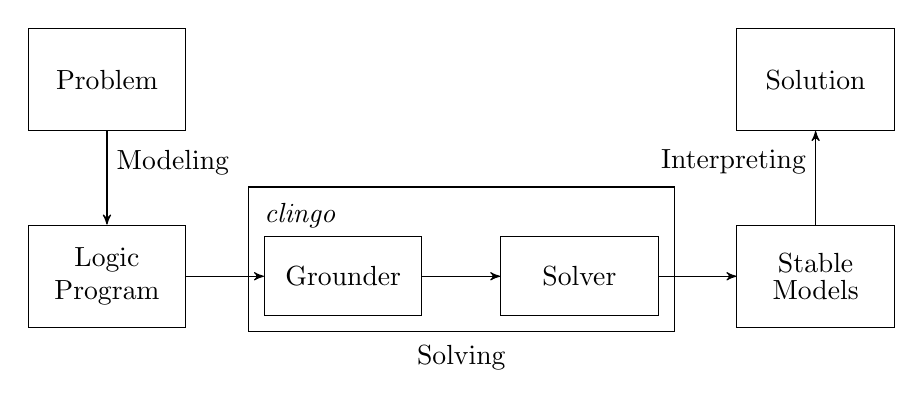
\begin{tikzpicture}[
      x=3cm,y=2.5cm,
      >=stealth',
      big box/.style={draw,minimum width=2cm,minimum height=1.3cm,inner sep=0},
      small box/.style={draw,minimum width=2cm,minimum height=1cm,inner sep=0},
      auto,
    ]
    \begin{scope}[every node/.style={big box}]
      \node (a) at (0,1) {Problem};
      \node (b) at (0,0) {\shortstack{Logic\\Program}};
      \node (e) at (3,0) {\shortstack{Stable\\Models}};
      \node (f) at (3,1) {Solution};
    \end{scope}
    \begin{scope}[every node/.style={small box}]
      \node (c) at (1,0) {Grounder};
      \node (d) at (2,0) {Solver};
    \end{scope}
    \node[above left, anchor=south west,inner sep=0,yshift=.1cm] (label) at (c.north west){\clingo};
    \node[draw,fit=(c) (d) (label),inner sep=.2cm] {};
    \path[->]
      (a) edge node [yshift=.2cm] {Modeling} (b)
      (b) edge (c)
      (c) edge node [swap,yshift=-.75cm] {Solving} (d)
      (d) edge (e)
      (e) edge node [yshift=.2cm] {Interpreting} (f);
  \end{tikzpicture}
  \caption{ASP solving process}%
  \label{fig:asp-in-a-nutshell}
\end{figure}

  The ASP solving process can be summarized by the steps depicted in \cref{fig:asp-in-a-nutshell}.
\end{itemize}

\section{Selected contributions}

\section{Overall contributions}

\begin{itemize}
  \item list all my contributions + how others are using them
\end{itemize}

\begin{itemize}
  \item check the Promotionsordnung for requirements
  \item my papers: \cites{%
    cafageiakakrlemarisc20a,%
    gekakasc17a,cakamosc19a,evjakasc19a,%
    rakaroscbogu18a,cakascsc18a,gekakaluobosroscscwa18a,%
    kascwa17a,jakaosscscwa17a,
    gejakascta16a,cakaossc16a,gekakalurosc16a,gekakaosscwa16a,%
    gehakalisc15a,gekakarosc15a,gekaobsc15a,gejajokasc15a,gekasc15a,%
    hokalisc14a,%
    kascsivi13a,gejokaobsascsc13a,%
    gegrkaobsasc12c,gekakasc12a,hokascsc12a,gegrkaobsasc12b,%
    gegrkasc11a,gekakaosscsc11a,gekaknsc11a,gekasc11b,gekakascsc11a,gekakasc11a,gekasc11c,gekakosc11a,gekakascsczi11a,%
    gekaosscth09a,gekakasc09a,scscgekakasc09a,elgegukakaliscscsc09a,%
    gekakaosscth08a}

\chapter{Publications}\label{sec:publications}

This section contains selected publications.

\includepub{%
  title={An ASP Semantics for Constraints Involving Conditional Aggregates},
  label={sec:publications:cafascwa20a},
  path={pub/cafascwa20a.pdf},
  authors={Pedro Cabalar, Jorge Fandinno, Torsten Schaub and Philipp Wanko},
  published_in={Frontiers in Artificial Intelligence and Applications Volume 325: ECAI 2020 664–671},
  bibentry={\cite{cafascwa20a}},
  doi={10.3233/FAIA200152}}

\includepub{%
  title={A Uniform Treatment of Aggregates and Constraints in Hybrid ASP},
  label={sec:publications:cafascwa20b},
  path={pub/cafascwa20b.pdf},
  authors={Pedro Cabalar, Jorge Fandinno, Torsten Schaub and Philipp Wanko},
  published_in={Proceedings of the Seventeenth International Conference on Principles of Knowledge Representation and Reasoning (2020) 193–202},
  bibentry={\cite{cafascwa20b}},
  doi={10.24963/kr.2020/20}}

\includepub{%
  title={Towards a Semantics for Hybrid ASP systems},
  label={sec:publications:cafascwa21a},
  path={pub/cafascwa21a.pdf},
  authors={Pedro Cabalar, Jorge Fandinno, Torsten Schaub and Philipp Wanko},
  published_in={To apear},
  bibentry={\cite{cafascwa21a}},
  doi={}}

\includepub{%
  title={Clingo goes Linear Constraints over Reals and Integers},
  label={sec:publications:jakaosscscwa17a},
  path={pub/jakaosscscwa17a.pdf},
  authors={Tomi Janhunen, Roland Kaminski, Max Ostrowski, Torsten Schaub, Sebastian Schellhorn and Philipp Wanko},
  published_in={Theory and Practice of Logic Programming 17 (2017) 872–888},
  bibentry={\cite{jakaosscscwa17a}},
  doi={10.1017/S1471068417000242}}


\includepub{%
  title={Computing Diverse Optimal Stable Models},
  label={sec:publications:roscwa16a},
  path={pub/roscwa16a.pdf},
  authors={Javier Romero, Torsten Schaub and Philipp Wanko},
  published_in={Schloss Dagstuhl-Leibniz-Zentrum fuer Informatik 52 (2016) 3:1–3:14},
  bibentry={\cite{roscwa16a}},
  doi={10.4230/OASIcs.ICLP.2016.3}}

\includepub{%
  title={teaspoon: Solving the Curriculum-Based Course Timetabling Problems with Answer Set Programming},
  label={sec:publications:bainkaokscsotawa18a},
  path={pub/bainkaokscsotawa18a.pdf},
  authors={Mutsunori Banbara, Katsumi Inou, Benjamin Kaufmann, Tenda Okimoto, Torsten Schaub, Takehide Soh, Naoyuki Tamura and Philipp Wanko},
  published_in={Annals of Operations Research 275 (2019) 3–37},
  bibentry={\cite{bainkaokscsotawa18a}},
  doi={10.1007/s10479-018-2757-7}}

\includepub{%
  title={Enhancing symbolic system synthesis through ASPmT with partial assignment evaluation},
  label={sec:publications:newascha17a},
  path={pub/newascha17a.pdf},
  authors={Dirk Abels, Julian Jordi, Max Ostrowski, Torsten Schaub, Ambra Toletti and Philipp Wanko},
  published_in={Design, Automation \& Test in Europe Conference \& Exhibition (2017) 306–309},
  bibentry={\cite{newascha17a}},
  doi={10.23919/DATE.2017.7927005}}

\includepub{%
  title={Exact Multi-Objective Design Space Exploration using ASPmT},
  label={sec:publications:newascha18b},
  path={pub/newascha18b.pdf},
  authors={Dirk Abels, Julian Jordi, Max Ostrowski, Torsten Schaub, Ambra Toletti and Philipp Wanko},
  published_in={Design, Automation \& Test in Europe Conference \& Exhibition (2018) 257–260},
  bibentry={\cite{newascha18b}},
  doi={10.23919/DATE.2018.8342014}}

\includepub{%
  title={Train Scheduling with Hybrid Answer Set Programming},
  label={sec:publications:abjoossctowa21a},
  path={pub/abjoossctowa21a.pdf},
  authors={Dirk Abels, Julian Jordi, Max Ostrowski, Torsten Schaub, Ambra Toletti and Philipp Wanko},
  published_in={Theory and Practice of Logic Programming 21 (2021) 317–347},
  bibentry={\cite{abjoossctowa21a}},
  doi={10.1017/S1471068420000046}}

\includepub{%
  title={Hybrid Metabolic Network Completion},
  label={sec:publications:frscscsiwa18a},
  path={pub/frscscsiwa18a.pdf},
  authors={Clémence Frioux, Torsten Schaub, Sebastian Schellhorn, Anne Siegel and Philipp Wanko},
  published_in={Theory and Practice of Logic Programming 19 (2019) 83–108},
  bibentry={\cite{frscscsiwa18a}},
  doi={10.1017/S1471068418000455}}



\section{Discussion}\label{sec:discussion}

We presented a comprehensive framework for computing diverse (or similar) solutions to logic programs with generic preferences
and implemented it in \asprin~2, available at~\cite{asprin}. %\comment{T: Make it available!}
To this end, we introduced a spectrum of different methods, among them, generalizations of existing work to the case of
programs with general preferences.
Hence, certain fragments of our framework provide implementations of the proposals in \cite{eiererfi13a,zhutru13a}.
While the latter had to resort to solver wrappers or even internal solver modifications,
\asprin\ heavily relies upon multi-shot solving that allows for an easy yet fine-grained control of reasoning processes.
Moreover, we provided several generic building blocks, such as 
\textit{maxmin} (and \textit{minmax}) preferences,
query-answering for programs with preferences,
preferences among optimal models,
and an automated approach for the guess and check methodology of~\cite{eitpol06a},
all of which are also of interest beyond diversification.
%
Finally, we took advantage of the uniform setting offered by \asprin~2 to conduct a 
comparative empirical analysis of the various methods for diversification.
Generally speaking,
there is a clear trade-off between performance and diversification quality, 
which allows for selecting the most appropriate method 
depending on the hardness of the application at hand.
%\comment{T: Last phrase is a bit weak\dots}
% \begin{itemize}
% \item System for diverse optimal models of logic program with preferences.
% \item Lifts previous approaches in ASP \cite{eiererfi13a} or with answer set optimization \cite{zhutru13a} to general preferences of \asprin.
% \item Variety of methods.
% \item Experimental evaluation shows that different methods differ wrt performance and diversity of solutions.
% \item There is a tradeoff between performance and diversity, which allows for selecting the most appropiate method at hand for the application at hand.
% \item Furthermore, four more general contributions to preferences: $maxmin$, automation of generate and test, query solving, and preferences over
% optimal models.
% \item Future work: Real world applications on DSS and TT.
% \item Future work: Apply SMT framework of \clingo\ 5. In \cite{eiererfi13a}, the modification of the solver was more efficient than ASP implementation.
%       We intend to do it in a principled (general?) way inside the new framework.
% \end{itemize}



%%% Local Variables: 
%%% mode: latex
%%% TeX-master: "paper"
%%% End: 

\input{sec/summary}

\appendix

\input{sec/grammar}

\backmatter
\bibliography{local,krr,procs}

\end{document}

%%% Local Variables:
%%% mode: latex
%%% TeX-master: t
%%% End:
